\section{Background and Related Works}
    \begin{figure}
        \centering
        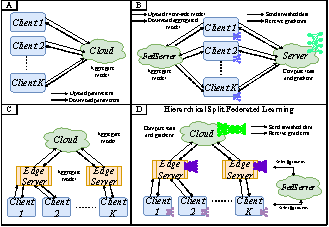
\includegraphics[width=\linewidth]{CVPR-2026/Figures/Related Works.pdf}
        \caption{Overview of FL paradigms. (A) Conventional FL exchanges full models with the cloud. (B) SplitFL transmits smashed data but depends on cloud gradients. (C) Hierarchical FL uses edge servers for intermediate aggregation. (D) Hierarchical SplitFL combines model splitting with hierarchical aggregation.}
        \label{fig:placeholder}
    \end{figure}
    Our work is positioned at the intersection of three key research areas aimed at solving the FL trilemma. The first, statistical heterogeneity, causes ``client drift" in FedAvg \cite{pmlr-v54-mcmahan17a}. Major solutions include regularization methods like FedProx \cite{dai2023tacklingFedProx}, drift-correction via control variates as in SCAFFOLD \cite{pmlr-v119-karimireddy20a}, and dynamic regularizers like FedDyn \cite{durmus2021federated}. A different approach, personalized FL (PFL), embraces heterogeneity. This is often achieved by decoupling models, as seen in FedPer \cite{arivazhagan2019federatedlearningpersonalizationlayers} and FedRep \cite{collins2021exploiting}, which train a shared representation but private heads. Other PFL strategies include pFedMe \cite{t2020personalized} using Moreau envelopes, and MOON \cite{9578660} using contrastive learning to align representations.

The second area, system heterogeneity, addresses client-side constraints. SL \cite{GUPTA20181, vepakomma2019split} solves this by partitioning the model, forcing clients to train only lightweight initial layers. To solve SL's sequential bottleneck, SFL \cite{thapa2022splitfed} was proposed to parallelize clients. A major alternative for handling computational diversity is HeteroFL \cite{diao2021heterofl}, which trains different-sized sub-models. System heterogeneity in terms of clients performing variable local work is addressed by methods like FedNova \cite{10.5555/3495724.3496362}, which normalizes local updates.

The third area tackles communication and scalability bottlenecks. Communication overhead is often reduced by model compression, such as quantization in QSGD \cite{alistarh2017qsgd} or sparsification in Deep Gradient Compression \cite{lin2017deep}. Another strategy is Federated Knowledge Distillation (e.g., FedDF \cite{lin2020ensemble}, FedGen \cite{venkateswaran2023fedgen}). The strategy we adopt, Prototype-Based FL \cite{tan2022fedproto}, exchanges lightweight prototypes, which both saves bandwidth and aids personalization. Separately, the single-server scalability bottleneck is solved by Hierarchical FL (HFL) \cite{rana2022hierarchical,9148862,9488756}, which introduces edge servers for intermediate aggregation and cloud workload reduction.

The existing literature has largely explored these techniques as separate solutions, each with their own limitations. For instance, SFL creates new server bottlenecks \cite{10980018} and incurs high communication costs from exchanging high-dimensional activations \cite{11091500, zhang2025amperecommunicationefficienthighaccuracysplit}, while FedProto can suffer from prototype drift under high heterogeneity \cite{bensiah2025feddpa, zhang2020personalized}. To our knowledge, no prior work has proposed a unified framework that synergistically integrates all three. Our H-SFP framework fills this gap. We use the HFL structure to solve SFL's scalability bottleneck and replace SFL's costly activation exchange with lightweight prototypes. 
It is critical to distinguish ours from methods like FedProto \cite{tan2022fedproto}. While FedProto uses prototypes as regularizers to align local training, H-SFP's prototypes are generative statistics ($\mu, \sigma$) used to synthesize new training data for the upper tiers, thereby enabling a fully decoupled, feed-forward training process. This yields a crucial synergistic benefit: the hierarchical, intragroup aggregation stabilizes the prototypes, mitigating drift. Therefore, our framework is simultaneously robust to non-IID data, computationally efficient for clients, and scalable to massive networks.

